\PassOptionsToPackage{unicode=true}{hyperref} % options for packages loaded elsewhere
\PassOptionsToPackage{hyphens}{url}
%
\documentclass[
]{article}
\usepackage{lmodern}
\usepackage{amssymb,amsmath}
\usepackage{ifxetex,ifluatex}
\ifnum 0\ifxetex 1\fi\ifluatex 1\fi=0 % if pdftex
  \usepackage[T1]{fontenc}
  \usepackage[utf8]{inputenc}
  \usepackage{textcomp} % provides euro and other symbols
\else % if luatex or xelatex
  \usepackage{unicode-math}
  \defaultfontfeatures{Scale=MatchLowercase}
  \defaultfontfeatures[\rmfamily]{Ligatures=TeX,Scale=1}
\fi
% use upquote if available, for straight quotes in verbatim environments
\IfFileExists{upquote.sty}{\usepackage{upquote}}{}
\IfFileExists{microtype.sty}{% use microtype if available
  \usepackage[]{microtype}
  \UseMicrotypeSet[protrusion]{basicmath} % disable protrusion for tt fonts
}{}
\makeatletter
\@ifundefined{KOMAClassName}{% if non-KOMA class
  \IfFileExists{parskip.sty}{%
    \usepackage{parskip}
  }{% else
    \setlength{\parindent}{0pt}
    \setlength{\parskip}{6pt plus 2pt minus 1pt}}
}{% if KOMA class
  \KOMAoptions{parskip=half}}
\makeatother
\usepackage{xcolor}
\IfFileExists{xurl.sty}{\usepackage{xurl}}{} % add URL line breaks if available
\IfFileExists{bookmark.sty}{\usepackage{bookmark}}{\usepackage{hyperref}}
\hypersetup{
  pdftitle={A Beautiful Start to a (CogSci) Paper},
  pdfauthor={Someone and Todd M. Gureckis},
  pdfborder={0 0 0},
  breaklinks=true}
\urlstyle{same}  % don't use monospace font for urls
\usepackage[margin=1in]{geometry}
\usepackage{graphicx,grffile}
\makeatletter
\def\maxwidth{\ifdim\Gin@nat@width>\linewidth\linewidth\else\Gin@nat@width\fi}
\def\maxheight{\ifdim\Gin@nat@height>\textheight\textheight\else\Gin@nat@height\fi}
\makeatother
% Scale images if necessary, so that they will not overflow the page
% margins by default, and it is still possible to overwrite the defaults
% using explicit options in \includegraphics[width, height, ...]{}
\setkeys{Gin}{width=\maxwidth,height=\maxheight,keepaspectratio}
\setlength{\emergencystretch}{3em}  % prevent overfull lines
\providecommand{\tightlist}{%
  \setlength{\itemsep}{0pt}\setlength{\parskip}{0pt}}
\setcounter{secnumdepth}{-2}
% Redefines (sub)paragraphs to behave more like sections
\ifx\paragraph\undefined\else
  \let\oldparagraph\paragraph
  \renewcommand{\paragraph}[1]{\oldparagraph{#1}\mbox{}}
\fi
\ifx\subparagraph\undefined\else
  \let\oldsubparagraph\subparagraph
  \renewcommand{\subparagraph}[1]{\oldsubparagraph{#1}\mbox{}}
\fi

% set default figure placement to htbp
\makeatletter
\def\fps@figure{htbp}
\makeatother

\usepackage{soul}
\usepackage{color}
\usepackage{cogsci}
\usepackage{apacite}
\usepackage[]{natbib}
\bibliographystyle{plainnat}

\title{A Beautiful Start to a (CogSci) Paper}
\author{Someone and Todd M. Gureckis}
\date{}

\begin{document}
\maketitle
\begin{abstract}
Put the abstract here
\end{abstract}

\hypertarget{introduction}{%
\section{Introduction}\label{introduction}}

Markdown supports \emph{italics}, \textbf{bold}, and
\textbf{\emph{bold\_italics}} style.

There are types of lists:

\begin{itemize}
\tightlist
\item
  something\\
\item
  something else\\
\item
  something else as well\\
\item
  fun
\end{itemize}

\citep{Gureckis2006} \citep{Chapman1967}

\hl{hi}

Or put another way:

\begin{enumerate}
\def\labelenumi{\arabic{enumi}.}
\tightlist
\item
  something\\
\item
  something else\\
\item
  something else as well
\end{enumerate}

A reference: \citep{Love2007}

\begin{itemize}
\tightlist
\item
  Item A

  \begin{itemize}
  \tightlist
  \item
    A sub list

    \begin{itemize}
    \tightlist
    \item
      What?
    \end{itemize}
  \item
    Another thing
  \end{itemize}
\item
  A fun thing
\end{itemize}

\hypertarget{i-am-a-subsection}{%
\subsection{I am a subsection}\label{i-am-a-subsection}}

Here is a figure that I will reference

\begin{figure}
\centering
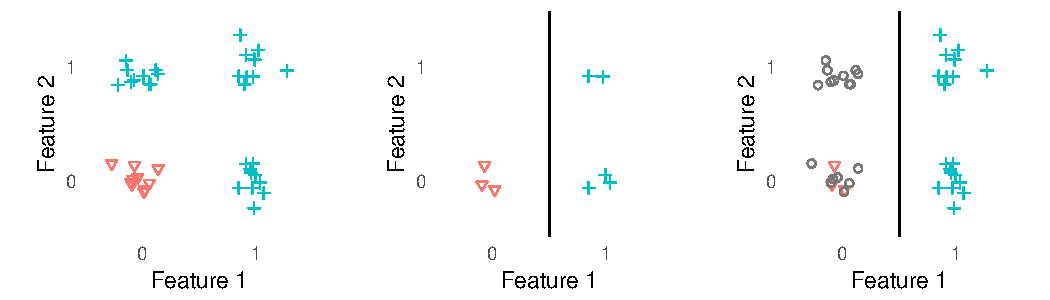
\includegraphics{figures/learning_trap.pdf}
\caption{This is my figure caption\label{fig:learning_trap}}
\end{figure}

\hypertarget{discussion}{%
\section{Discussion}\label{discussion}}

\renewcommand\refname{References}
  \bibliography{library.bib}

\end{document}
